\documentclass[../sparc.tex]{subfiles}
\graphicspath{{\subfix{../images/}}}
\begin{document}

%%%%%%%%%%%%%%%%%%%%%%%%%%%%%%%%%%%%%%%%%%%%%%%%%%%%%%%%%%%%%%%%%%%%%%%%%%%%%%%%
\section{Аналоговые порты}
\label{section:analog-ports}

На отладочной плате Arduino присутствуют так называемые \emph{аналоговые порты},
которые позволяют считывать аналоговый сигнал.  На плате они подписаны как
\texttt{A0}, \texttt{A1}, и т.д. Если цифровые порты рассчитаны на цифровой
сигнал, который может быть в двух состояниях - 0 В или 5 В, то аналоговые,
соответственно, рассчитаны на аналоговый, непрерывный сигнал, который может
принимать любые значения от 0 до 5 В.

В качестве первого эксперимента мы попробуем вывести аналоговый сигнал на
компьютер с аналогового порта, который никуда не подключен.

В коде будем использовать функцию \texttt{analogRead}:

\begin{minted}{cpp}
void setup() {
  Serial.begin(9600);
}

void loop() {
  // Получаем значение с аналогового порта 0
  int value = analogRead(A0);

  Serial.println(value);

  delay(100);
}
\end{minted}

Еслы мы посмотрим на монитор порта в Arduino IDE, то увидим, что сигнал
принимает значения, которые на вид совершенно случайны.  Тем не менее, мы можем
на них влиять -- если поднесём руку, то скорее всего увидим, что сигнал
изменился.  Означает ли это, что у нас открылись супер-способности и нам пора
записываться в лигу супер-героев?  К сожалению, нет -- но всё же мы только что
открыли способность в Arduino считывать электромагнитный шум, который в обычной
жизни, как правило, невидим для нас.

Есть несколько способов ``увидеть'' этот шум в обыденной жизни.  Например, можно
настроить радио на частоту между радио-станциями, и услышать ``шипение'' из
динамика.  Пример такого шума показан на рис. \ref{fig:white-noize}.

\begin{figure}[ht]
  \centering
  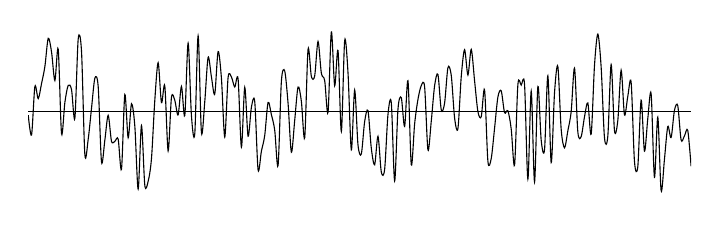
\begin{tikzpicture}[samples=200, domain=0:5*360]
    \begin{axis}[
        width=10cm, height=4cm,
        enlarge x limits=false,
        xtick=\empty,
        axis lines*=middle,
        hide y axis
      ]
      \addplot [no markers, smooth] {sin(x)+rand*2};
    \end{axis}
  \end{tikzpicture}
  \caption{Белый шум.}
  \label{fig:white-noize}
\end{figure}

Как бы странно это не звучало, но есть разные ``цвета'' шума: ``белый'',
``розовый'', ``красный'', ``фиолетовый'' и ``серый''.  Шумы различных ``цветов''
различаются спектром сигнала, и характеристика ``цвета'' дана по аналогии со
спектром видимого света.  В нашем случае мы рассматриваем ``белый'' шум, который
и дал название этой главе.

``Белый'' шум -- это сигнал, составляющие которого распределены равномерно по
всему диапазону используемых частот.  Если ``белый'' шум воспроизвести через
динамик, чтобы мы могли его услышать, то мы сможем услышать, что все слышимые
нами частоты звука в нём распределены равномерно -- иными словами, мы услышим
просто ``ш-ш-ш-ш'' из динамика или аудио-колонок.

\note{Изображение \ref{fig:white-noize} сгенерировано в момент создания
  электронной версии книги в формате PDF, и в разных версиях книги оно будет
  различаться.  Это вызвано тем, что для генерации изображения используется
  генератор случайных чисел, а случайность в компьютере обычно берётся из
  непредсказуемости окружающего мира -- в частности, как уже говорилось выше,
  источником такой непредсказуемости является ``Белый шум''.}

В случае с Arduino, эти шумы улавливаются самой схемой, и преобразуются в набор
чисел определённого диапазона.

Данный электромагнитный фон постоянно присутствует вокруг нас; у него есть много
разных источников.  Во-первых, шум создаёт человеческая цивилизация в целом --
телевизионные и радиовышки; базовые станции, обеспечивающие работу мобильных
телефонов; сами телефоны, передающие данные по беспроводным сетям и многое
другое.  Во-вторых, существуют совершенно естественные, природные, источники
радиоволн -- например, некоторые виды звёзд производят очень мощный радиосигнал.

Для более удобного просмотра этого сигнала удобно воспользоваться ``плоттером по
последовательному соединению'', доступного из меню ``Инструменты'' (``Tools'') --
таким образом, вы можете увидеть график, подобный \ref{fig:white-noize}.

\experiment{0}{Попробуйте поднести мобильный телефон к Arduino.  Как изменится
  сигнал?}

\experiment{1}{Подключите порт \texttt{A0} сначала к земле (порту ``GND''),
  потом отключите его и подключите \texttt{A0} к порту 5V на Arduino.  Что
  происходит с сигналом при этих действиях?}

Есть ли какое-то применение этому ``шуму''?  Оказывается, да.  Благодаря своей
непредсказуемости, он может быть использован в качестве источника случайных
чисел -- что бывает полезно например при разработке игр, о чём будет рассказано в
последующих главах книги.

\end{document}
